\section{Face Fusion Algorithm}
\label{sec:algorithm}

Given a source face image $I_s$ and a target face image $I_t$, our goal is to generate a new face image $I_f$ which fuses the facial features of the two faces into a natural-looking face.
Our method consists of two steps: (1) \emph{geometric alignment}, which re-arranges the facial landmarks of the target face according to the source face, and (2) \emph{appearance fusion}, which fuses two faces in the gradient domain. Fig.~\ref{fig:pipeline} shows the pipeline of our approach.




\comments{
It is necessary to calculate the location and the size of the facial part from each face image. With the help of the facial landmarks \cite{fld}, it is quick to perform this step. But only knowing the location and the size of two faces is not enough. We need to know where are the eyes, nose and other parts of two faces. Different faces have different face features, some people have a big nose while others with a small one. Some people's nose is closer to eyes while others' nose is farther to eyes. Still, with the help of facial landmarks, we know exactly the distribution of face features.


By aligning two faces, we know the features on one face and their corresponding features on the other face. Then, we fuse two faces from parts to parts.
}

\begin{center}
    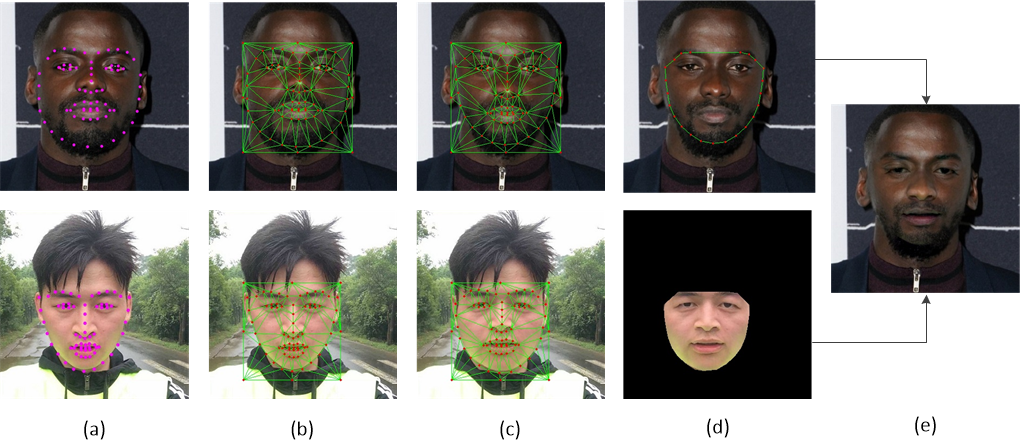
\includegraphics[width=4.8in]{images/pipeline.png}
    \fcaption{Pipeline of our approach. (a) Perform facial landmark detection on two faces. (b) Triangulate two faces according to the facial landmarks. (c) Calculate new facial landmarks by interpolating two groups of facial landmarks, warp two faces according to the new facial landmarks. (d) Reconstruct gradients on facial part for fused face . (e) Fuse features of source face into target face by seamless cloning. \cxj{Choose two figures that are more beautiful. Mark the source and target image.}}
    \label{fig:pipeline}
\end{center}

\subsection{Face alignment}


\mdf{While the two face areas are different in scale, position, and orientation in $I_s$ and $I_t$, we first align the two faces according to their facial landmarks. }
%
There are many techniques to detect facial landmarks \cite{fld2,fld3,fld4,fld}. We adopt \cite{fld}. It is an much faster method exist;
%It is implemented in Dlib.
\cxj{Why do you choose this method?}

In Fig.~\ref{fig:pipeline}(a), with the landmarks of two faces, the bounding boxes of two faces are calculated. But two bounding boxes can not be directly compared.
We reshape the bounding boxes of two faces into square by stretching the shorter side of bounding boxes and get bounding squares of two faces.
With the bounding squares of two faces, we know the sizes of two faces.
\cxj{Why don't you directly compute the transformation between two bounding boxes?}
%
%
Before we triangulate a face according to facial landmarks, we need make sure that the transition from the background to the face is natural. If we interpolate two groups of facial landmarks directly, the profile of the interpolated facial landmarks would be different from the facial landmarks of the target face.
\cxj{why do you have to consider the background area?}
%
So we add eight points into the facial landmarks to help triangulate the faces. In Fig.~\ref{fig:face-warpping}(b), the eight points lie on the boundary of a square. The square is generated by enlarging the bounding square of the face. Four points are on the corners of the square and the others are on the mid points of sides of the square.
%
The center point and the side length of bounding square of source face are denoted as $\mathbf{c}_s$ and $l_s$.
The center point and side length of bounding square of target face are denoted as $\mathbf{c}_t$ and $l_t$.
%
The indexes of facial landmarks on the face denoted as $i \in \{1...N\}$, $N$ is the number of facial landmarks.
For each point $\mathbf{p}_s$ inside the bounding square of source face, we calculate its corresponding location on the target face $\vb{p}_t$ by following mapping function:
%
\begin{equation}
\label{eq:trans-point}
\vb{p}_t=\frac{l_t}{l_s}(\vb{p}_s-\vb{c}_s) + \vb{c}_t.
\end{equation}

The facial landmarks we need to triangulate on the source face and the target face are denoted as $\vb{F_{s}}$(the red points on the face image in second row of Fig.~\ref{fig:pipeline}(b)) and $\vb{F_{t}}$(the red points on the face image in first row of Fig. 1(b)) respectively.
The facial landmarks of the output face are denoted as $\vb{F_n}$. It can be calculated by interpolating $\vb{F_s}$ and $\vb{F_t}$. With these new facial landmarks, we can create a new face structure. For each point in $\vb{F_s}$, $\vb{F_t}$ and $\vb{F_n}$, they are denoted as $\vb{F}_{\vb{s}_i}$, $\vb{F}_{\vb{t}_i}$ and $\vb{F}_{\vb{n}_i}$ respectively.

\begin{equation}
\label{eq:inp-point}
\vb{F}_{\vb{n}_i} = \alpha \cdot f(\vb{F}_{\vb{s}_i}) + (1-\alpha) \cdot \vb{F}_{\vb{t}_i},
\end{equation}

where $\alpha$ controls which face structure we prefer more. If $\alpha$ is small, the new face structure would look more like the target face. It means that the profile of the new face and the distribution of the new face features would look more like the target face.

After triangulating two faces according to $\vb{F_s}$ and $\vb{F_t}$ using Delaunay Triangulation, we get two sets of triangles from the source face and the target face, denoted as $\vb{T_s}$ and $\vb{T_t}$. The corresponding triangles of two faces are not of the same shape because of different facial landmarks. What we need to do is to make sure the shape of corresponding triangles of two faces are the same. We warp the triangles in $\vb{T_{t}}$ one by one to the $\vb{T_{n}}$. Then we warp $\vb{T_s}$ to $\vb{T_n}$ in a similar way.
\cxj{1. How to warp the triangular mesh? Warping each triangle independently?}

In Fig.~\ref{fig:pipeline}(c), the source face and the target face are warped according to an common interpolated mesh. The sizes and the locations of their bounding squares are different at each face image, but the shapes of the corresponding triangles of two faces are the same.
\cxj{Given two meshes, there should be just one transformation to alignment.}

After warping two faces, we have two faces of the same structures and the same distributions of face features. But the sizes and the locations of their bounding squares are different. We extract the bounding square area of the source face, scale and translate the area to the same size and location of the bounding square of the target face. The extracted face witch is translated and resized is shown in Fig.~\ref{fig:face-warpping}(b).

As we can see from the Fig.~\ref{fig:face-warpping}, the triangles of the source face and the target face are exactly at the same location and of the same shapes and sizes. The purpose of our task is to fuse the features of the source face into the target face. So we need to know the profile of the source face. In Fig.~\ref{fig:face-warpping}(c), the yellow outline is generated from the facial landmarks. What we want is that all the pixels inside the yellow outline are from the face. In fact, some pixels may come from the background. So we get the blue outline by shrinking the profile a little. Inside the blue outline, all the pixels are from the facial part. The area inside the blue outline is $\Omega$, where $\Omega$ stands for the facial part we are going to fuse.

\cxj{This should be in the face alignment part which computes the geometric transformation.}


\begin{center}
    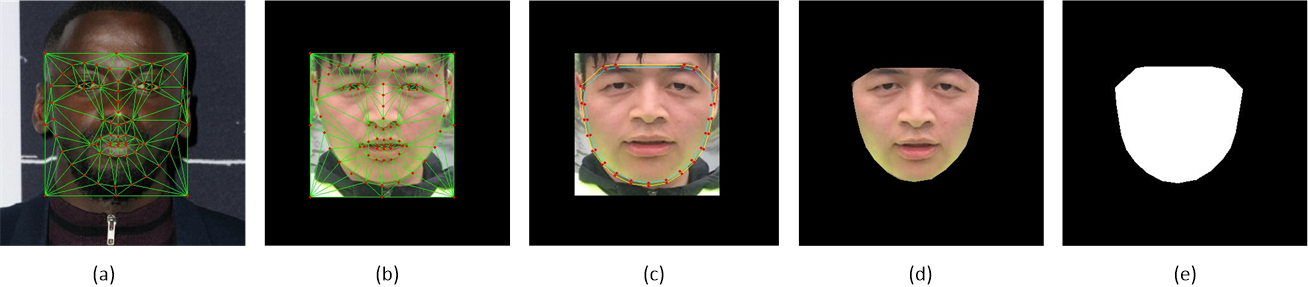
\includegraphics[width=4.8in]{images/extract.png}
    \fcaption{(a) The target face warped according to $\vb{F_n}$. (b) The warped source face after being translated and scaled. (c) Yellow outline is generated from the landmarks of the warped source face, light blue outline is shrank a little from the yellow profile. (d) Facial part of the warped source face that inside $\Omega$. (e) Facial mask. \cxj{Why do you need to show two outlines in (c)? They should be the same.}}
    \label{fig:face-warpping}
\end{center}


\subsection{Gradient-based Fusion}
\label{sec:fusion}

The target face and the source face are shown in Fig.~\ref{fig:face-warpping}(a) and Fig.~\ref{fig:face-warpping}(b). We fuse the gradients of two faces, recover the face from the fused gradients by seamless clone.

The gradients of the source face is denoted as $g_s$. The gradients of target face is denoted as $g_t$. There are three ways we tried to construct the guidance field.

For the first way, the guidance field $g_1$ is generated  by linearly combinating $g_s$ and $g_t$:

\begin{equation}
\label{eq:gradient-linear}
g_1 = \beta g_s+(1-\beta) g_t.
\end{equation}

For the second way, at each point in $\Omega$, guidance field $g_2$ retain the stronger gradients in $g_s$ or in $g_t$:

\begin{equation}
\label{eq:gradient-mixed}
for\ all\ \vb{x} \in \Omega, g_2(\vb{x})=\left\{
\begin{aligned}
g_s(\vb{x}) &&{if |g_s(\vb{x})|>|g_t(\vb{x})|}\\
g_t(\vb{x}) &&{else}\\
\end{aligned}
\right.
\end{equation}

For the third way, we define $g_3$ by linearly combination of $g_d$ and $g_t$:

\begin{equation}
\label{eq:gradient-shed}
g_3 = \beta \cdot g_d+(1-\beta) \cdot g_t,
\end{equation}


where $g_d$ is:

\begin{equation}
\label{eq:gradient-mixed-sub}
for\ all\ \vb{x} \in \Omega, g_d(\vb{x})=\left\{
\begin{aligned}
g_t(x) &&{if \ |g_s(\vb{x})|< \theta_1 \ and \ |g_t(\vb{x})|< \theta_2}\\
g_s(x) &&{else}\\
\end{aligned}
\right.
\end{equation}


$g_d$ contains the stronger gradients of the $g_s$ and weaker gradients of $g_t$. If $g_s(\vb{x})$ is smaller than the threshold $\theta_1$ and $g_t(\vb{x})$ is smaller than the threshold $\theta_2$, then $g_d(\vb{x})$ keeps the gradient from $g_t$ at point $x$. So it contains main features of the source face and the part of the lightning condition of the target face. Fig.~\ref{fig:shed}(a) and Fig.~\ref{fig:shed}(b) are facial parts of the target face and the source face. They share the same profile and distribution of features, Fig.~\ref{fig:shed}(c) shows which parts of $g_d$ are come from $g_t$ or $g_s$. For all $\vb{x} \in \Omega$ and for each channel, if $g_d(\vb{x})$ is come from $g_s(\vb{x})$, then the corresponding part in Fig.~\ref{fig:shed}(c) is brighter.

\cxj{All these ways to create gradient field can be found in \cite{pie}, you only need one sentence "the gradient field is calculated in the same way with \cite{pie}."}

Finally, we use $g$ to recover the face we want on the target face image by seamless clone.
\begin{center}
    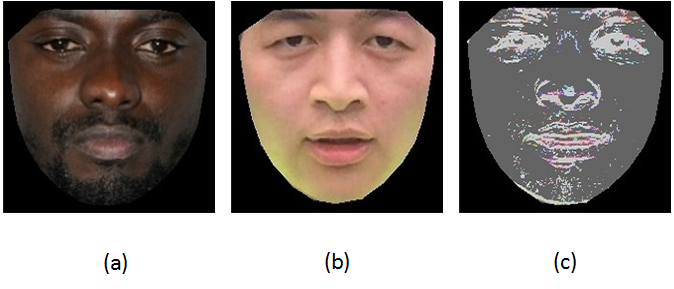
\includegraphics[width=3in]{images/labelmasks.png}
    \fcaption{(a) Facial part of target face. (b) Facial part of the source face. (c) A mask indicates which part of $g_d$ are come from $g_s$ or $g_t$.}
    \label{fig:shed}
\end{center}
